\chapter{Research Methodology}

\section{Choice of technology}
Even though most tools for the semantic web are written in Java, some open source libraries for Python have become availabe in recent years \cite{w3java}. Python then became an easy choice for extracting data from the sources and transforming it to LOD. For publishing the data, we chose to host a Sparql Endpoint using Apache Fuseki and use LodView to dynamically generate an HTML representation of the dataset based on the Sparql endpoint. A major benefit of this, is that Fuseki also provide access to a reasoner, ensuring that the published data is as rich as possible. Fuseki and LodView are deployed using Apache Tomcat, along with a reverse proxy in Apache HTTP server in order to make them publicy available on the internet. For representing the data as a graph we have utilized Lod Cloud Draw and \textbf{XXXXXXXXXXXXXXXXXXXX.js}

\vspace{5mm}

Although Apache Fuseki does function as a public SPARQL endpoint, security issues led us to want to hide this interface, and rather provide a separate public endpoint using YASGUI, which also gives a some extra functionality like map plotting of the query results.

\vspace{5mm}

For handling the automatic workflow scheduling, we opted for Apache Airflow as we had learned about this in class.

\vspace{5mm}

The technology choice we struggled the most with, was for the HTML representation. Here we experimented with several frameworks like Pubby and Loddy before landing on LodView, which provided all the functionality we wanted.

\section{Data collection process}
Statens vegvesen (Norwegian Public Roads Administration) \cite{statensvegvesen} provides an API for their parking data in JSON format. As the API only gives access to subsets of the data, we have created a program that fetches the complete dataset and creates a single JSON file.

\vspace{5mm}

This data is fed to a program that combines our RDF schema as seen in Appendix \ref{appendix:ontology} and the parking data, generating RDF triples in a RDF/XML file format. The program additionally uses data from the Norwegian postal and logistics company Bring \cite{bring} to match postal codes from Statens vegvesen's data with Norwegian municipality codes. These codes are then linked with Wikidata \cite{wikidata} using their SPARQL endpoint.

\vspace{5mm}

In our RDF schema, we inherit and reuse vocabularies we have found in the ontologies provided at Schema-org \cite{schema-org} and MobiVoc \cite{schema-mobivoc}.


\section{System architecture}

\begin{figure}[H]
	\centering
	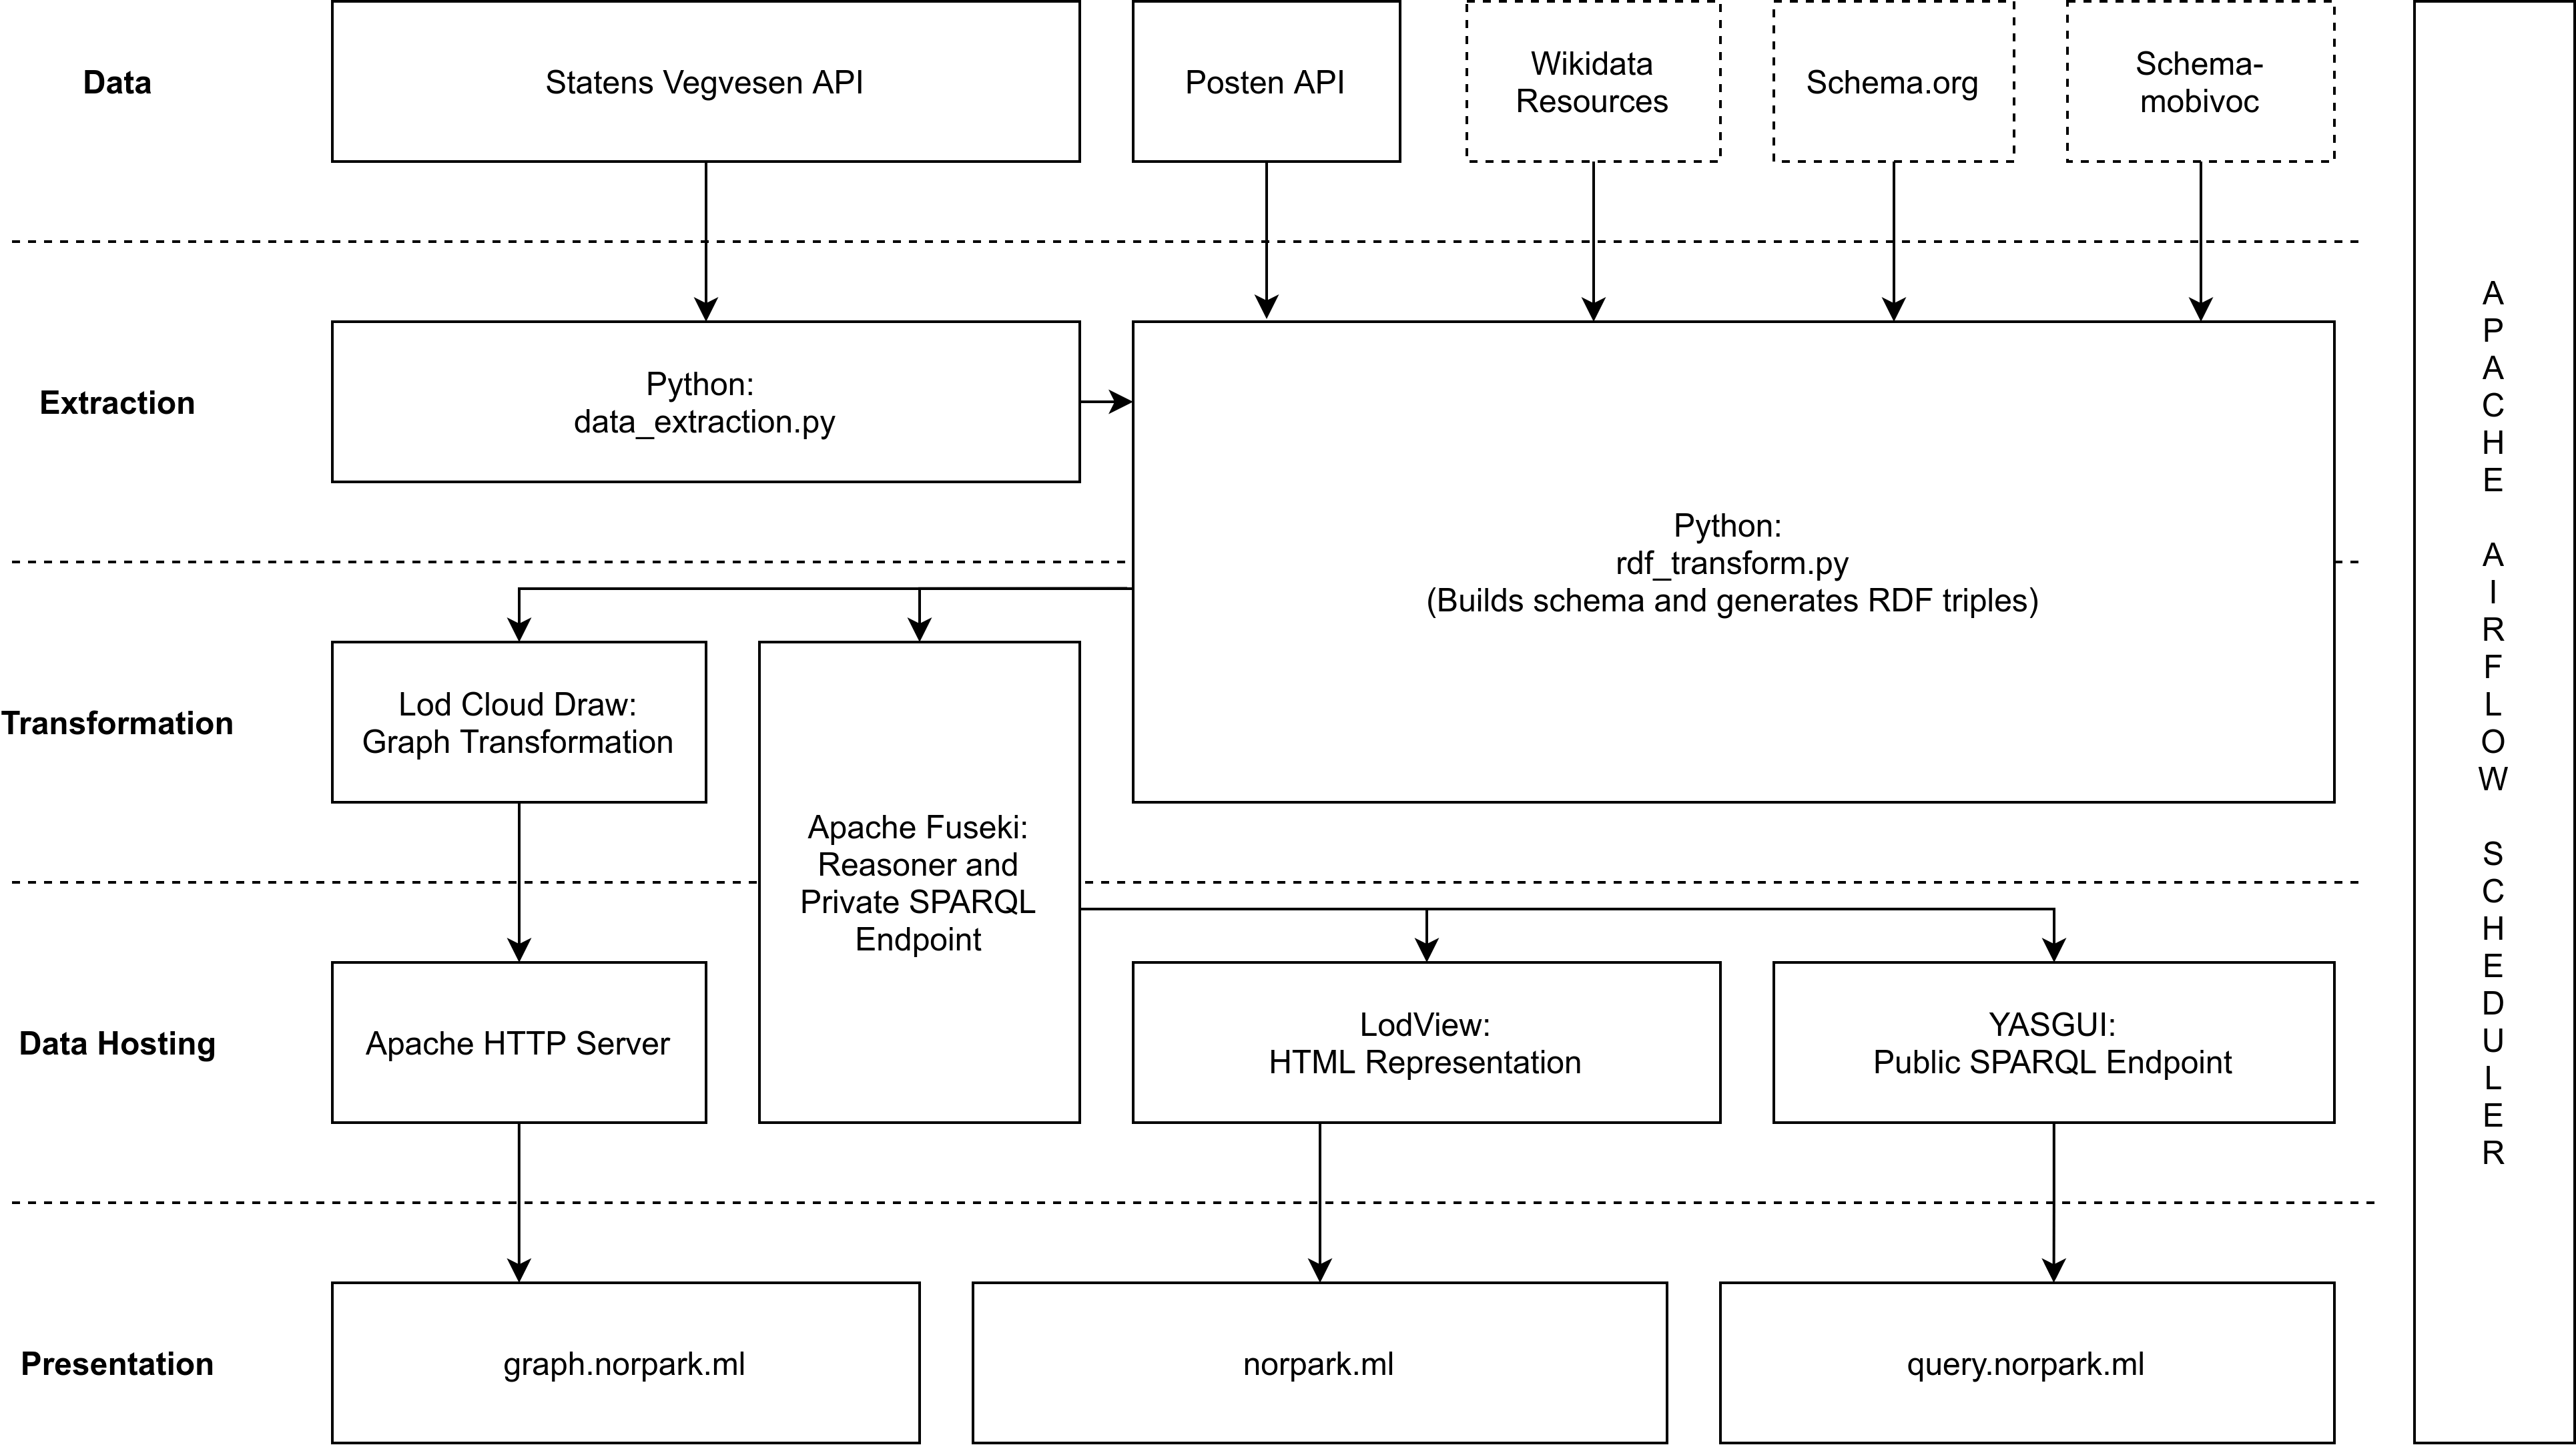
\includegraphics[width=\linewidth]{figures/system-architecture.png}
	\caption{The system architecture}
\end{figure}



